\documentclass[12pt,letterpaper]{article}
\usepackage{graphicx}
\usepackage{ifpdf}

\usepackage{multicol}
\usepackage{tikz}

\usepackage{amssymb}
\usepackage{amsmath}

\usepackage{hyperref}
% \usepackage{cite}

\usepackage[backend=bibtex]{biblatex}
\bibliography{bibliografia} 

\hypersetup{
    colorlinks=true,
    linkcolor=black,
    citecolor = black,
%     filecolor=magenta,      
    urlcolor=black,
%     pdftitle={GSP Toolbox Manual},
    bookmarks=true
%     pdfpagemode=FullScreen,
}

\usepackage[spanish]{babel}

\usepackage{fancyhdr}
 
\pagestyle{fancy}
\fancyhf{}
\rhead{Isaac Ayala Lozano\\194520009 \hspace{2 em}   \textbf{\#2}}
\lhead{}
\fancyfoot[R]{\thepage}

\begin{document}

\section{Tarea \#05 - Métodos numéricos}

\subsection{Runge-Kutta}

Se implementó un algoritmo en Jupyter para resolver \emph{ecuaciones diferenciales ordinarias} empleando el método Runge-Kutta de cuarto orden. El modelo matemático para el método Runge-Kutta fue tomado de \cite{andasari}.

\begin{equation}
 y_{i+1} = y_i + \frac{h}{6} (k_1 + 2k2_2 + 2 k_3 + k_4)
\end{equation}


\begin{equation}
 \begin{split}
  k_1 &= f(x_i, y_i)\\
  k_2 &= f(x_i + \frac{h}{h}, y_i + \frac{h}{2}k1)\\
  k_3 &= f(x_i + \frac{h}{h}, y_i + \frac{h}{2}k2)\\
  k_4 &= f(x_i+h, y_i+h k_3)\\
 \end{split}
\end{equation}


Se evaluó el algoritmo para las funciones $\sin(x)$ y $\cos (x)$ con múltiples condiciones iniciales. Los detalles de la simulación se pueden observar en la tabla \ref{table: simulation}.


 \begin{table}[h]
 \centering
 \begin{tabular}{cc}  
 Tamaño de paso (h) & 0.1\\
 Intervalo de integración (t) & [0, 2$\pi$] \\
 Condiciones de inicio ($x_0$) & [-3, 3]
  \end{tabular} 
\caption{Condiciones de la simulación.}
 \label{table: simulation}
 \end{table}




Al observar el comportamiento de las ecuaciones en las figuras \ref{fig: rk sin} y \ref{fig: rk cos}, se pueden identificar valores a los cuales ambas funciones tienden a estabilizarse. Para el caso de la función seno, existen tres valores a los que tiende la función: $-\pi, 0, \pi$. Para el caso de la función coseno los valores son $\frac{\pi}{2}, -\frac{5\pi}{2}$


\begin{figure}[h]
 \centering
 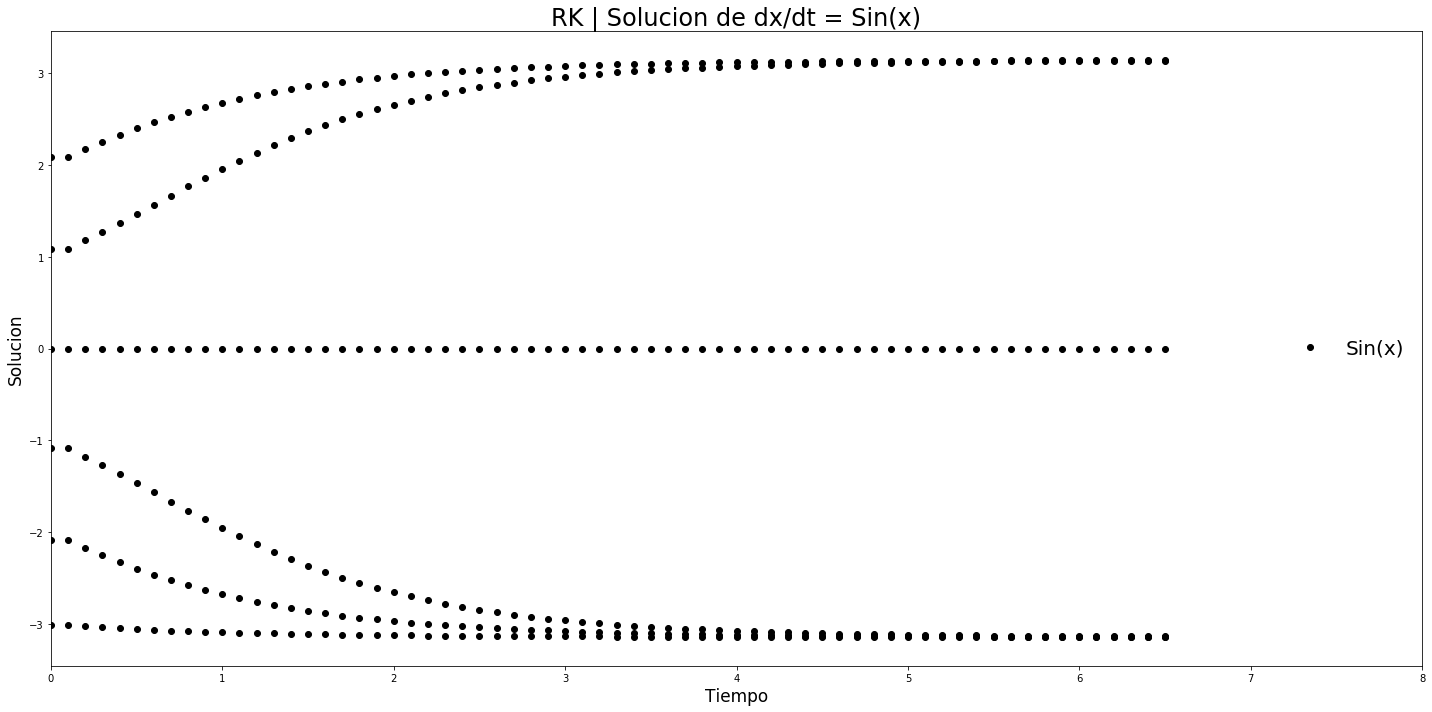
\includegraphics[scale=0.25]{img/rk_sin.png}
 % rk_sin.png: 1432x712 px, 72dpi, 50.53x25.12 cm, bb=0 0 1432 712
 \caption{Resultados de evaluación empleando el método de Runge Kutta.}
 \label{fig: rk sin}
\end{figure}

\begin{figure}[h]
 \centering
 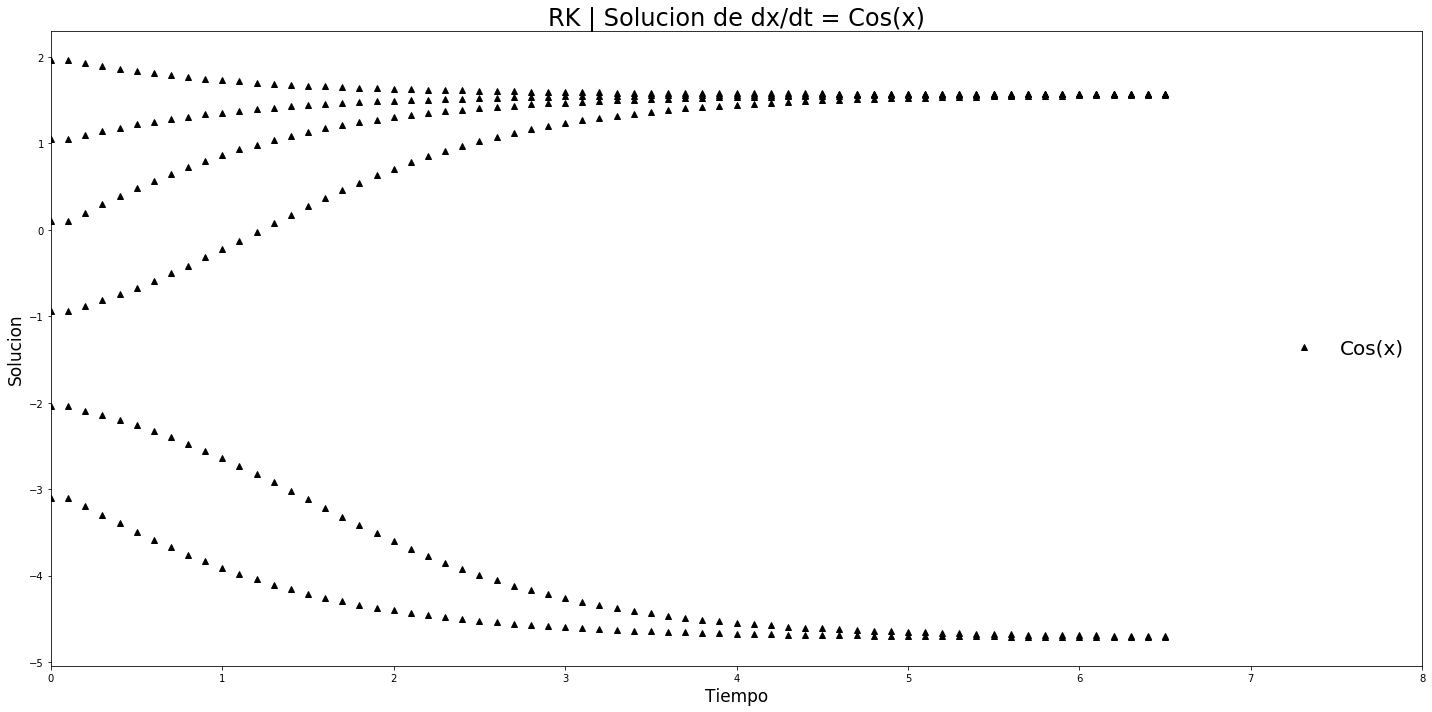
\includegraphics[scale=0.25]{img/rk_cos.png}
 % rk_sin.png: 1432x712 px, 72dpi, 50.53x25.12 cm, bb=0 0 1432 712
 \caption{Resultados de evaluación empleando el método de Runge Kutta para la función seno.}
 \label{fig: rk cos}
\end{figure}

\pagebreak

\subsection{lsoda}
El kernel de SageMath, empleado dentro de Jupyter, incluye los solucionadores numéricos de SciPy. Uno de estos solucionadores es  \emph{lsoda} que fue adaptado de la librería provista por FORTRAN.
Se evaluó el solucionador para las funciones seno y coseno, empleando las mismas 
condiciones de simulación que el solucionador Runge-Kutta. Los resultados de dichas simulaciones se muestran en las figura \ref{fig: lsoda sin} y \ref{fig: lsoda cos}.
Se observa que de igual manera, las funciones tienden a los mismos valores que
el solucionador Runge-Kutta.


\begin{figure}[hb]
 \centering
 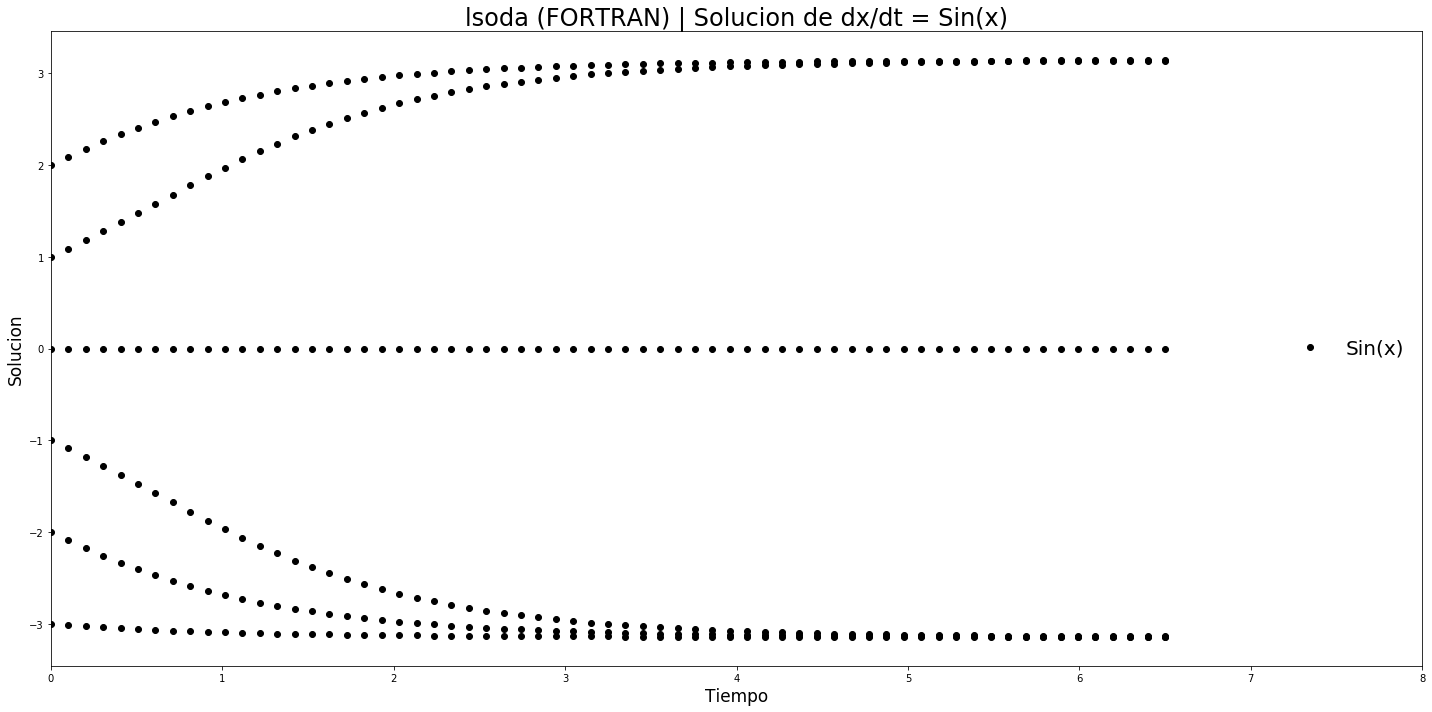
\includegraphics[scale=0.2]{img/lsoda_sin.png}
 % rk_sin.png: 1432x712 px, 72dpi, 50.53x25.12 cm, bb=0 0 1432 712
 \caption{Resultados de evaluación empleando el solucionador numérico \emph{lsoda} para la función seno.}
 \label{fig: lsoda sin}
\end{figure}

\begin{figure}[hb]
 \centering
 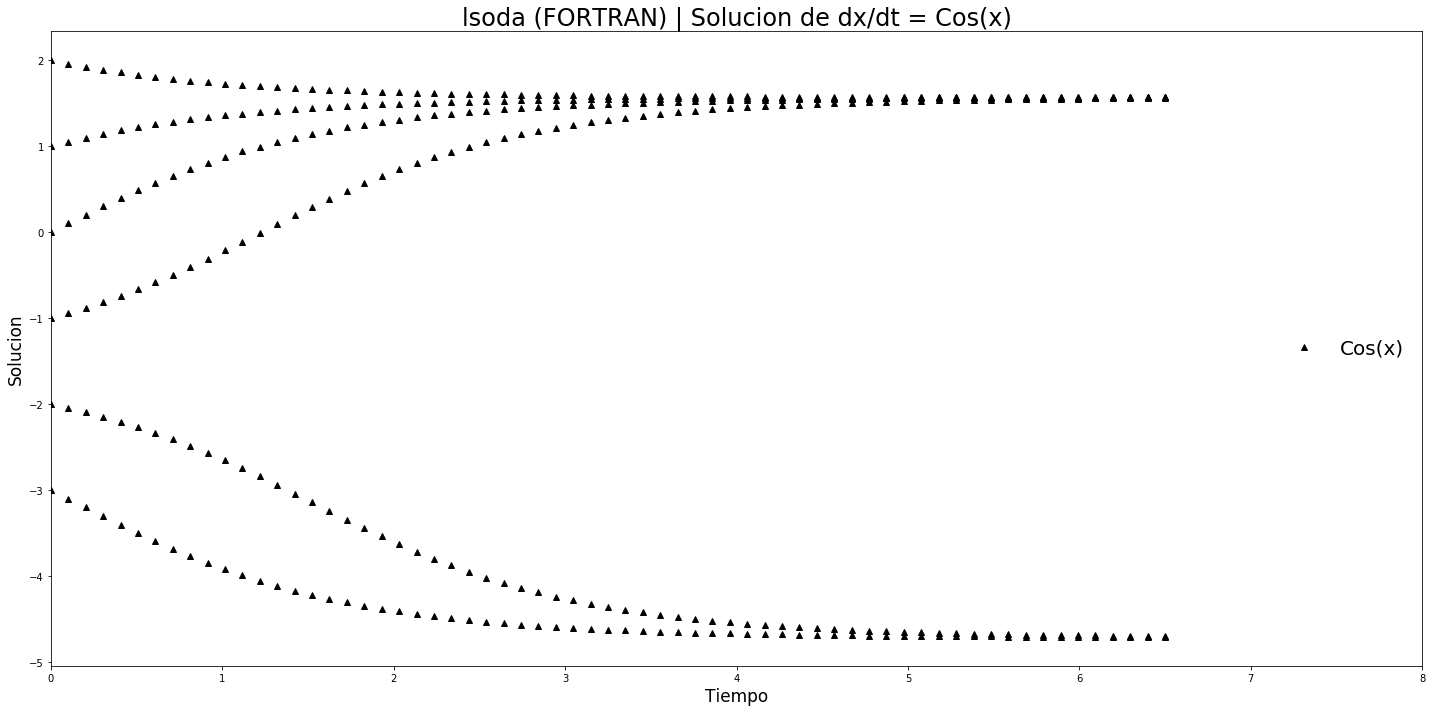
\includegraphics[scale=0.2]{img/lsoda_cos.png}
 % rk_sin.png: 1432x712 px, 72dpi, 50.53x25.12 cm, bb=0 0 1432 712
  \caption{Resultados de evaluación empleando el solucionador numérico \emph{lsoda} para la función coseno.}
 \label{fig: lsoda cos}
\end{figure}

\pagebreak

\subsection{Comparación}

Para la comparación de los solucionadores se tomó exclusivamente el comportamiento de las funciones con las condiciones de inicio $x(0) = 3, \dot{x}(0)=3$. Se observa que la función tiende a un valor único conforme el tiempo t tiende a infinito. Es posible identificar diferencias entre solucionadores
al inspeccionar los primeros puntos de evaluación en las figuras \ref{fig: lsoda rk sin} y \ref{fig: lsoda rk cos}.

\begin{figure}
 \centering
 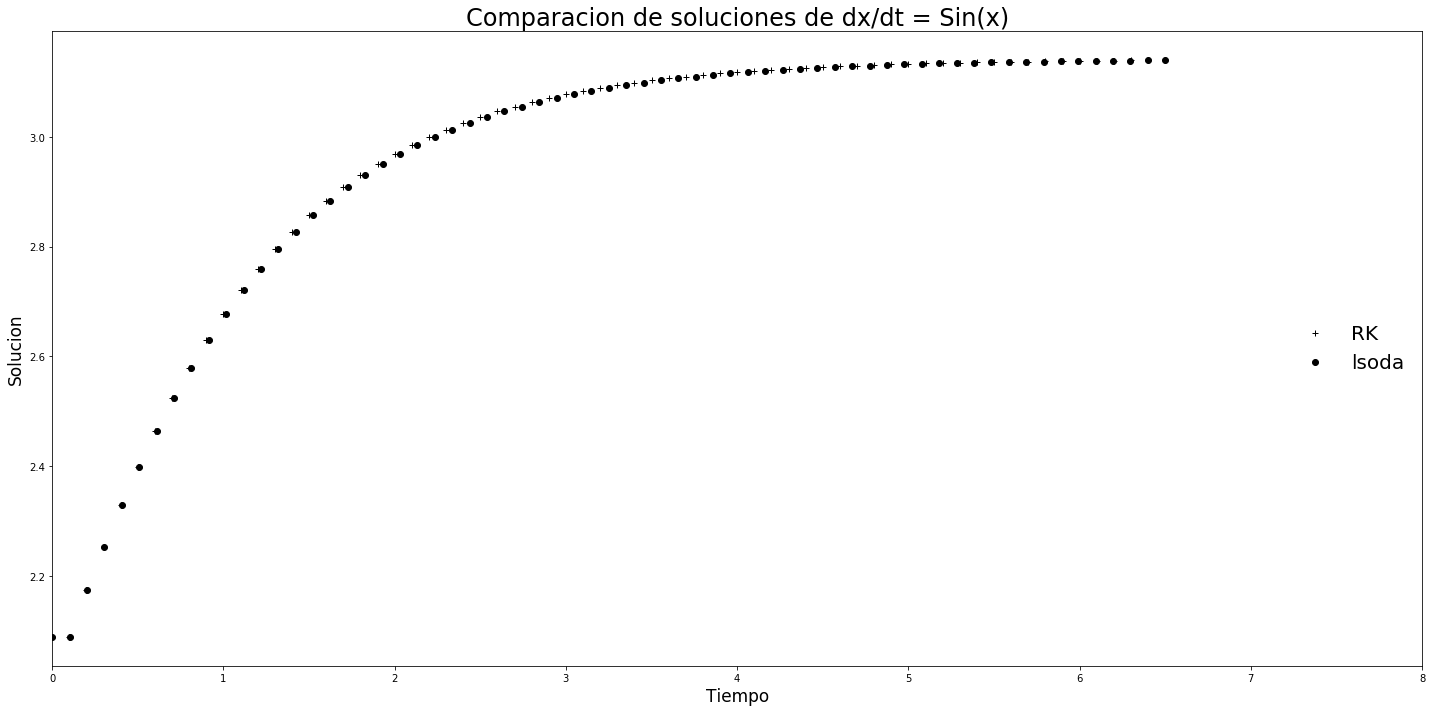
\includegraphics[scale=0.25]{img/lsoda_rk_sin.png}
 % rk_sin.png: 1432x712 px, 72dpi, 50.53x25.12 cm, bb=0 0 1432 712
 \caption{Comparación de resultados entre solucionadores para la función seno.}
 \label{fig: lsoda rk sin}
\end{figure}

\begin{figure}
 \centering
 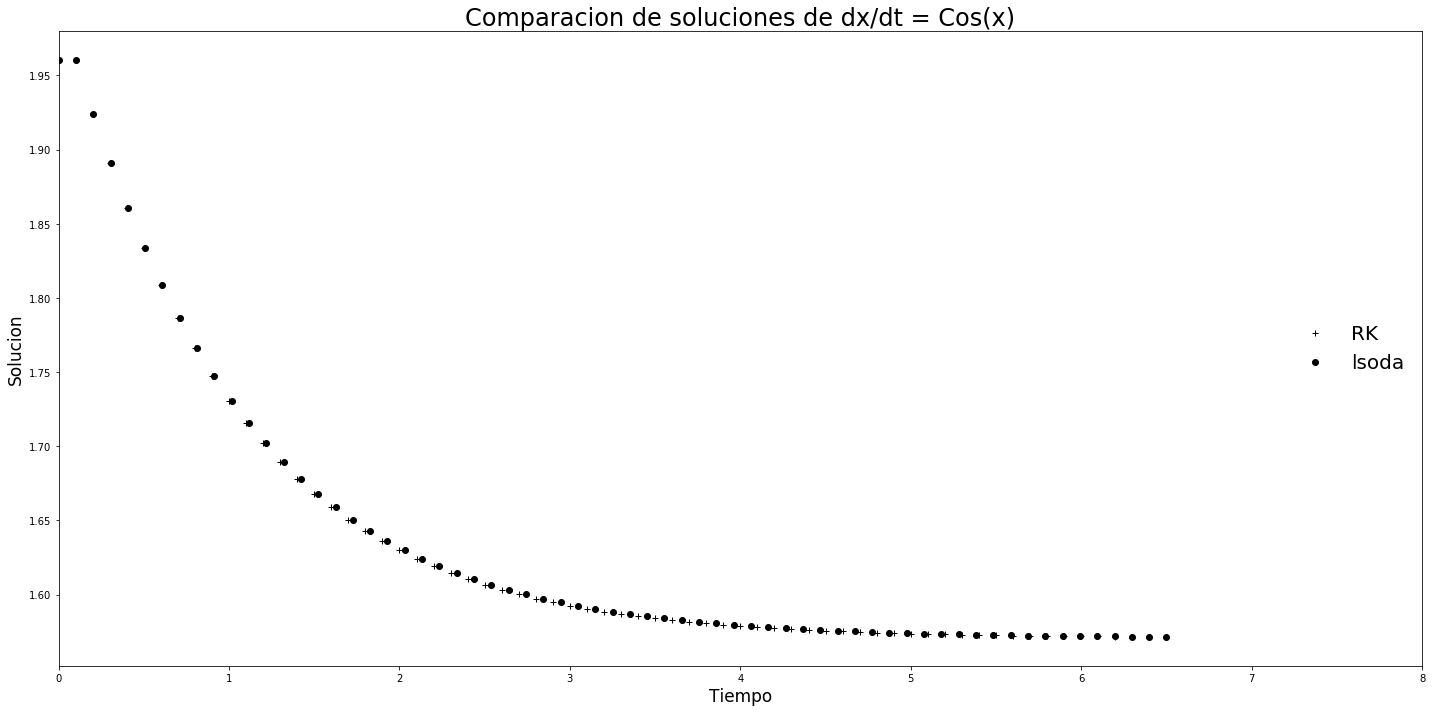
\includegraphics[scale=0.25]{img/lsoda_rk_cos.png}
 % rk_sin.png: 1432x712 px, 72dpi, 50.53x25.12 cm, bb=0 0 1432 712
 \caption{Comparación de resultados entre solucionadores para la función coseno.}
 \label{fig: lsoda rk cos}
\end{figure}

\printbibliography
\end{document}
